\begin{figure}
    \begin{center}
    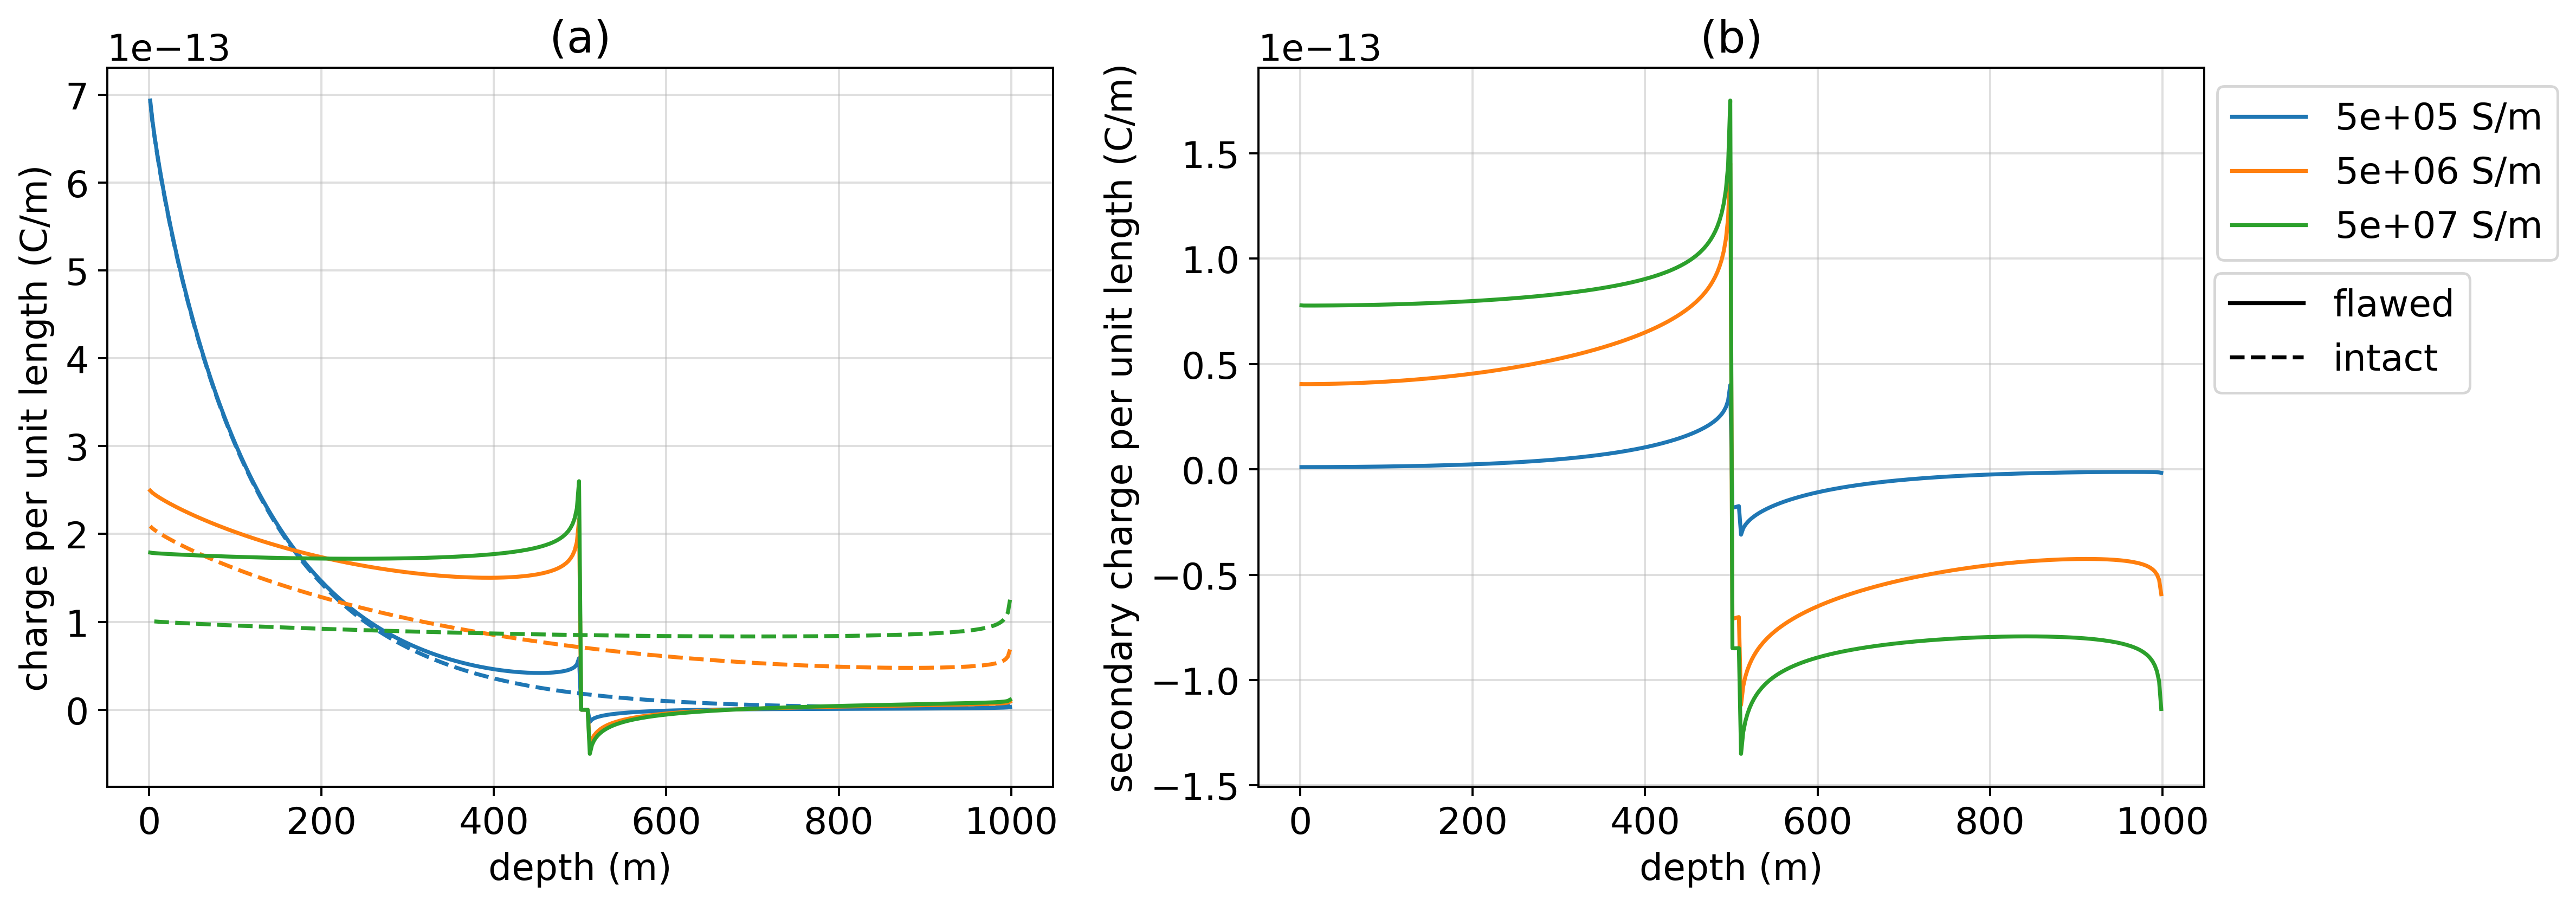
\includegraphics[width=\textwidth]{figures/dc_casing/casing_charge_sigma_casing.png}
    \end{center}
\caption{
    (a) Charge along the length of wells with three different
    conductivities (each indicated by a different color in the legend).
    The intact wells are denoted with dashed lines and the flawed wells
    are denoted with solid lines.
    (b) Secondary charge along the flawed and short wells. The primary is
    defined as the electric field due to the 1000 m long intact well. The return electrode
    is 2000 m away from the well.
}
\label{fig:casing_charge_sigma_casing}
\end{figure}
